% Chapter 9

\chapter{Analysis of 2016 raw multiplicities} % Chapter title

\label{ch:raw} % For referencing the chapter elsewhere, use \autoref{ch:name}

The 2006 SIDIS COMPASS hadron multiplicities results, based on data taken with an isoscalar target ($^6$LiD), do not constrain fermly the strange quark fragmentation function.
With the analysis of new data taken on pure proton target (lH$_2$), the results will provide a new set of equations linking the multiplicities with the fragmentation functions but still involving the same quark fragmentation functions we are interested in. The fact that the proton and deuteron data can be fitted together will add constrains to the fragmentation function extraction.
In order to perform this kind of study, one need a precision of 5 to 7\% on the multiplicities.

The analysis is performed on COMPASS data recorded in 2016 using a 160 GeV muon beam incident on a proton target (lH$_2$). Five weeks of the 2016 data are analyzed (dubbed P07, P08, P09, P10 and P11).

%----------------------------------------------------------------------------------------

\section{Method of extraction}

The method of extraction of the multiplicities follow several steps. For each selection steps,
a list of cuts is applied on both geometrical and physical quantities. First the DIS events are selected
and then the SIDIS events (hadrons) are selected. For the DIS event selection, a study on the target radius
had to be made in order to determine the optimal value for the target cut. When the event selection is done, the hadrons have to be identified between pions, kaons and protons and the identification has to be corrected according to the RICH detection efficiency and purity in a process called unfolding. The obtained raw multiplicities are then binned and corrected with the detector acceptance. The general event reconstruction codes for COMPASS are used. A personal analysis code is developed to study the SIDIS channel and select pion or kaon production events.

In the following, the number of residual events after each cut will be given between parentheses next to each cut.
When the number is not specified, it can mean that the cut was done in a pre-analysis or that the recovery of the number is too complex due to the transversal implementation of the cut in the code (e.g. for the $\nu$ cut).

The analysis is performed on COMPASS data recorded in 2016 using a 160 GeV muon beam incident on a pure proton target (lH$_2$).
Five periods of the 2016 data are analyzed : P07, P08, P09, P10 and P11.

%------------------------------------------------

\section{DIS event selection}

For the DIS event selection ($\mu p \rightarrow \mu X$), the following list of cuts is applied :
\begin{enumerate}
  \item Events with Best Primary Vertex (53.8 M events, 100\%)
  \item Events with reconstruted scattered muon (53.8 M events, 100\%)
  \item Events with primary interaction in the target material, target radius cut (explained in Section \ref{}, 22.7 M events, 42.1\%)
  \item Events with energy of beam muon energy in range [140 GeV, 180 GeV] (22.7 M events, 42.1\%)
  \item Events with a well reconstructed beam track (so-called 'BMS cut') (20.8 M events, 38.6\%)
  \item Events with $\chi^2$/ndf $<$ 10 for a well reconstructed beam track (20.8 M events, 38.6\%)
  \item Events with muon beam trajectory crossing entirely the target cell (20.0 M events, 37.2\%)
  \item Events with $\chi^2$/ndf $<$ 10 for a well reconstructed scattered muon track (20.0 M events, 37.2\%)
  \item Events with Z coordinate of the first measured hit of scattered muon $<$ 350 cm ($Z_{SM1}$) (19.9 M events, 37.1\%)
  \item Events with Middle, Ladder, Outer or LAST trigger (19.9 M events, 37.1\%)
  \item Events with $Q^2>1$ (GeV/c)$^2$ (DIS validity, 13.9 M events, 25.8\%)
  \item Events with $0.1 < y < 0.9$ (6.3 M events, 11.7\%)
  \item Events with $5 < W < 17$ GeV/c$^2$ (6.3 M events, 11.6\%)
  \item Events with $0.004 < x < 0.4$ (6.3 M events, 11.6\%)
  \item Events with $\nu$ cut
\end{enumerate}

The cut on the kinematic variable $\nu$ was implemented to reject events that contain hadrons outside of the measured
momentum range of 12 - 40 GeV/c. The criteria is defined by :
\begin{equation}
  \nu_{max} = \frac{\sqrt{(p^2_{max}+m^2_h)}}{z_{max}}
\end{equation}
\begin{equation}
  \nu_{min} = \frac{\sqrt{(p^2_{min}+m^2_h)}}{z_{min}}
\end{equation}

where $p_{max}$ (resp. $p_{min}$) is the hadron momentum limit of 40 GeV/c (resp. 12 GeV/c), $z_{max}$ (resp. $z_{min}$)
is the upper (resp. lower) value of the $z$-bin and $m_h$ is the mass of the considered hadron.

%------------------------------------------------

\section{Target cut evaluation}

The target in 2016 is long and not straight ('banana shaped', Fig. \ref{}), with a shape not easily reproducible in Monte-Carlo. The Monte-Carlo target is only a cylinder that was tilted by an angle extracted from the real data target. This angle correspond to the angle between the upstream and downstream ends of the target. Of course due to its 'banana shape' in reality, the description of the target in Monte-Carlo is not reaching 100\% fidelity. After the radial cut on the real data target (1.9 cm radius and $y$ = 1.2 cm), the residual volume, which is the volume of the real data target remaining after intersection with the Monte-Carlo target, is of n\% (Fig. \ref{pic:Target}). This then brings a systematic error on the multiplicities that I wanted to avoid. To this end, I devised three different solutions :

\begin{figure}[!h]
	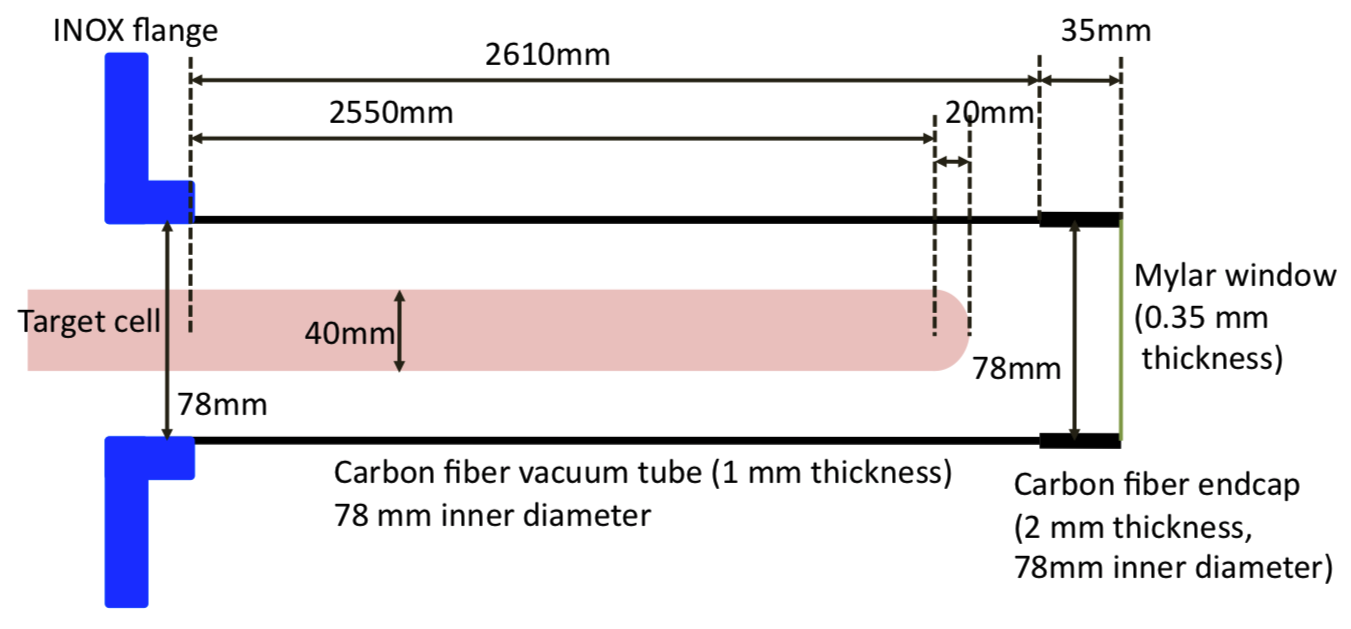
\includegraphics[scale=0.4]{./gfx/Target.png}
	\caption{Left is a ($y$,$z$) view of the real data (blue) and the Monte-Carlo target (red), $z$ being the direction of propagation of the beam. The actual cut used in the analysis corresponds to the intersection of both real data target (red) and Monte-Carlo target (blue) volumes. Right is a sketch showing approximately how much we lose by doing such cut.}
	\label{pic:Target}
\end{figure}

\begin{enumerate}
  \item Cut more severely on the radius of the real data target (1.7 cm radial cut) to reduce the  residual volume to zero.
  \item Do a simultaneous cut on the real data target and on the Monte-Carlo target to only keep the intersection between the two volumes.
  \item Do a better description of the target in the Monte-Carlo by using several cylinder volumes and fuse them together to increase the fidelity of the Monte-Carlo target description with respect to the real data one.
\end{enumerate}

The last solution was evacuated due to time constraints allowed by the analysis and my thesis, however I think this is the solution we should choose in the future to maximise the efficiency of the analysis from a statistic point of view.
The first two solutions were in competition and had the same spirit : cut more in the data target to avoid any systematic bias between real data target and Monte-Carlo target. I chose the second one, a simultaneous cut on both target, as it was the one that was discarding less target volume, thus maximising statistics. In Fig. \ref{} you can see the volume that survive such cut.

%------------------------------------------------

\section{Downstream target vertex distribution}

We discovered when looking at vertex distribution for hadrons and comparing data with Monte-Carlo that there was a deficit of vertices in the downstream part of the target (between -100 and -70 cm, Fig. \ref{VertexDrop}). We saw this phenomenon both in data and Monte-Carlo however it was more stressed in data than in Monte-Carlo. After investigation, we discovered that, both in data and Monte-Carlo, there were a high number of hadrons that have their track not attached to the best primary vertex in a 2 mm-radius circle around the best primary vertex (Fig. \ref{CircleHadron}). This circle is only visible in the downstream part of the target while in the upstream part it is non-existant.

\begin{figure}[!h]
	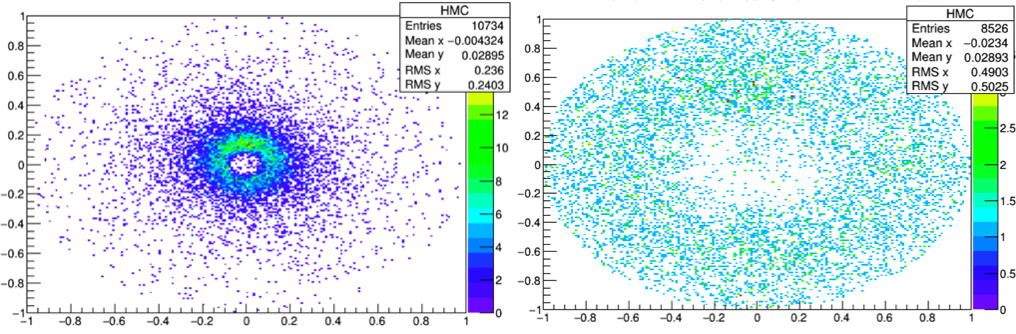
\includegraphics[scale=0.45]{./gfx/CircleHadron.png}
	\caption{Both plots are representing the relative distance to the best primary vertex of the extrapolated position of the unattached hadrons to the vertex position. Left the plot is done in the downstream part of the target, right in the upstream part. The left plot shows an important amount of particles in a 2 mm-radius circle around the vertex while the right plot does not.}
	\label{CircleHadron}
\end{figure}

This issue probably needs a thorough investigation of how the reconstruction is done in this case. As time was in short supply, we decided to go with a rescue procedure to reattach these hadrons to the best primary vertex. All the hadrons in a circle of radius 2 mm around the best primary vertex are considered as if they were attached to it (considering they have a track ID and a momentum associated). With this procedure we were able to cover for the loss of hadron in the last part of the target (Fig. \ref{VertexDrop}). One can fear that with such procedure I attach back some hadrons that should not be attached. Here I bring two answers : a part of these 'bad' hadrons are hadrons reconstructed without associated momentum and are thus non-eligible to this rescue procedure. Another part are hadrons that will then be cut out by hadron cut, especially by the RICH entrance angle cut. A last part of these 'bad' hadrons will effectively be part of the hadron sample but I consider the 'bad' hadron fraction to be negligible compared to the 'good' hadrons fraction, thus no systematic is applied concerning this rescue procedure. Again, this method is only temporary and this problem should be investigated more thoroughly in the future as it seems it is a long term problem within COMPASS reconstruction procedure.

\begin{figure}[!h]
	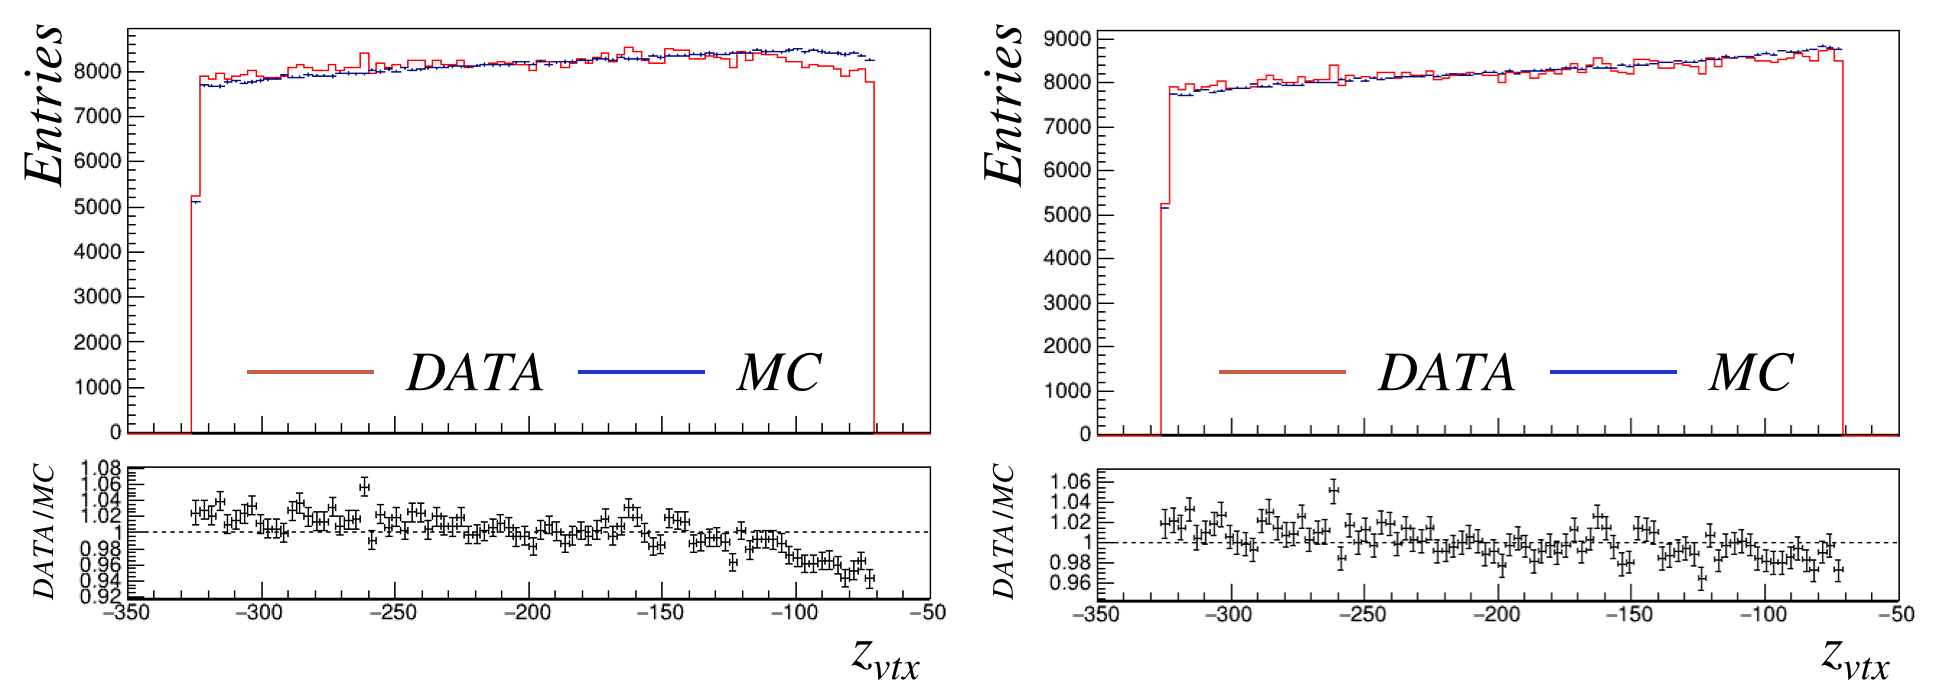
\includegraphics[scale=0.45]{./gfx/VertexDrop.png}
	\caption{One expects the vertex distribution for hadrons to increase with $z_{vtx}$ due to the apparatus acceptance. However in the left plot there is a drop both in data and Monte-Carlo of the number of vertices. In the right plot, after the rescue procedure, the drop has disappeared. The rescue procedure also reconciles data and Monte-Carlo.}
	\label{VertexDrop}
\end{figure}

%------------------------------------------------

\section{Hadron selection}

For the hadron selection ($\mu p \rightarrow \mu hX$), the following list of cuts is applied :
\begin{enumerate}
  \item Particle is not a scattered muon (15.2 M hadrons, 100\%)
  \item Maximum radiation length cumulated along all the trajectory < 15 radiation lengths (14.9 M hadrons, 98.3\%)
  \item $\chi^2$/ndf $<$ 10 for the hadron track (14.6 M hadrons, 96.1\%)
  \item Z coordinate of the first measured hit < 350 cm (14.6 M hadrons, 95.9\%)
  \item Z coordinate of the last measured hit > 350 cm (14.6 M hadrons, 93.6\%)
  \item $0.01 < \theta_{RICH} < 0.12$ (at RICH entrance, 9.5 M hadrons, 62.3\%)
  \item $x^2_{RICH} + y^2_{RICH} > 25$ cm$^2$ (rejection of RICH pipe) (9.3 M hadrons, 61.5\%)
  \item $12 < p_h < 40$ GeV/c (2.5 M hadrons, 16.5\%)
  \item $0.2 < z < 0.85$ (1.9 M hadrons, 13.1\%)
\end{enumerate}

%----------------------------------------------------------------------------------------

\section{Particle Identification with RICH detector}

The $\pi$ and $K$ particle identification (PID) is performed by the RICH detector.

The method used for the RICH particle identification is described in \ref{}. The idea is the following : when a particle
is detected, six likelihood functions are calculated ($\pi$, $K$, $p$, $e$, $\mu$ and the background) and are then
compared to make the particle identification. The evaluation is done separately for pions, kaons and protons. The largest
value corresponds to the maximal probability. The method is improved by looking further to $LH(2^{nd})$ which is the second
highest value of the four compared likelihood values ($\pi$, $K$, $p$ and the background). The electron and muon likelihood
are not considered in the assignment of $LH(2^{nd})$ as in the chosen momentum range (12 to 40 GeV/c) the RICH detector can
not be used to efficiently distinguish electrons from $\pi$.

All $\pi$, $K$ and $p$ probabilities are needed for the unfolding.


\begin{enumerate}
  \item Pion selection
  \begin{itemize}
    \item $LH(\pi) > 0$
    \item $LH(\pi) > LH(K)$, $LH(p)$ and $LH(bg)$.
    \item $\frac{LH(\pi)}{LH(2^{nd})}>1.02$
    \item $\frac{LH(\pi)}{LH(bg)}>2.02$
  \end{itemize}
  \item Kaon selection
  \begin{itemize}
    \item $LH(K) > 0$
    \item $LH(K) > LH(\pi)$, $LH(p)$ and $LH(bg)$.
    \item $\frac{LH(K)}{LH(2^{nd})}>1.08$
    \item $\frac{LH(K)}{LH(bg)}>2.08$
  \end{itemize}
  \item Proton selection
  Three cases are considered depending on the momentum $p_{h}$ of the particle and are defined but the kaon threshold ($\simeq 8.9$ GeV/c)
  and proton threshold ($\simeq 17.95$ GeV/c)
  \begin{enumerate}[(a)]
    \item Kaon threshold $< p_{h} \leq$ proton threshold - 5 GeV/c
	  \begin{center}
		  \begin{tabular}{c|c}
		    \hline
		     $p$ & $\bar{p}$ \\
		    \hline
				\multicolumn{2}{c}{Not to be a $\pi$ or $K$} \\
		    $\frac{LH(\pi)}{LH(bg)} < 2.2$ & $\frac{LH(\pi)}{LH(bg)} < 2.1$ \\
		    $\frac{LH(K)}{LH(bg)} < 2.9$ & $\frac{LH(K)}{LH(bg)} < 2.8$ \\
		    \hline
				\multicolumn{2}{c}{or all $LH$ = 0} \\
				\hline
		  \end{tabular}
		\end{center}
    \item $p_{h} >$ proton threshold + 5 GeV/c
    \begin{itemize}
      \item $LH(p) > 0$
      \item $LH(p) > LH(\pi)$, $LH(K)$ and $LH(bg)$.
      \item $\frac{LH(p)}{LH(2^{nd})}>1$
    \end{itemize}
    \item Proton threshold - 5 GeV/c $< p_{h} <$ proton threshold + 5 GeV/c
    \begin{itemize}
      \item Using (a) and (b) simultaneously.
    \end{itemize}
  \end{enumerate}
\end{enumerate}

%----------------------------------------------------------------------------------------

\section{RICH unfolding based on efficiency matrices}

The performance of the RICH is not perfect : neither in terms of efficiency nor in terms
of purity.

The unfolding procedure is needed to correct the yield of identified hadrons for this imperfection.
In order to perform this correction, the RICH actual performance is evaluated from real data. The result of
this evaluation is presented through RICH performance matrices, $M_{RICH}$, binned in momentum
and angle :

\begin{itemize}
  \item $p_h$ \{12,13,15,17,19,22,25,27,30,35,40\} GeV/c
  \item $\theta$ \{0.01,0.04,0.12\} rad
\end{itemize}

The 3-by-3 matrices $M_{RICH}$ give a relation between the vector of true hadron $T_h$ and the vector of
identified hadron $I_h$

\begin{equation}
\begin{bmatrix}
I_{\pi} \\
I_K \\
I_p
\end{bmatrix}
=
\begin{bmatrix}
\epsilon(\pi \rightarrow \pi) & \epsilon(K \rightarrow \pi) & \epsilon(p \rightarrow \pi)\\
\epsilon(\pi \rightarrow K) & \epsilon(K \rightarrow K) & \epsilon(p \rightarrow K) \\
\epsilon(\pi \rightarrow p) & \epsilon(K \rightarrow p) & \epsilon(p \rightarrow p)
\end{bmatrix}
\begin{bmatrix}
T_{\pi} \\
T_K \\
T_p
\end{bmatrix}
\end{equation}

The coefficients of the $M_{RICH}$, $\epsilon(t \rightarrow i)$, are the probabilities that a true hadron
$t$ is identified as a hadron of type $i$. These probabilities have been determined as described in \ref{RICH_NOTE}.

The true hadrons have obtained by inverting the performance matrices (Eq. \ref{richmat}) :

\begin{equation}
  \overrightarrow{T_h} = M^{-1}_{RICH}\overrightarrow{I_h}
	\label{richmat}
\end{equation}

\begin{table}[!h]
  \caption{\label{HadNum} Number of identified pions, kaons, and protons for the 5 periods before and after unfolding.}
  \centering
  \begin{tabular}{lcccccc}
    \hline
     & $\pi^+$ & $\pi^-$ & $K^+$ & $K^-$ & $p$ & $\bar{p}$ \\
    \hline
    Identified & 953970 & 789480 & 253045 & 153440 & 131066 & 60705 \\
    Unfolded & 976213 & 814685 & 255132 & 150775 & 124221 & 52014 \\
    \hline
  \end{tabular}
\end{table}

%----------------------------------------------------------------------------------------

\section{Kinematic binning}

The raw multiplicities are evaluated in bins of the Bjorken variable $x$, the muon energy fraction carried
by the virtual photon $y$ and the virtual photon energy fraction carried by final state hadron $z$. They
are calculated with the following formula :

\begin{equation}
  \frac{dM^h(x,y,z)}{dz}=\frac{1}{N^{DIS}_{Events}(x,y)}\frac{dN^{DIS}_{h}(x,y,z)}{dz}
\end{equation}

where $N^{DIS}_{Events}$ is the number of DIS events and $N^{DIS}_{h}$ is the number of
hadrons after RICH unfolding. As in practise, the multiplicities are measured in bins of
x (9 bins), y (5 bins) and z (12 bins), the calculated multiplicities can be expressed as :

\begin{equation}
  M^h_{raw}(x,y,z) = \frac{N^{DIS}_{h}(x,y,z)/\delta z}{N^{DIS}_{Events}}
\end{equation}

where $\delta z$ is the width of the z bin. For the multiplicities extraction, the binning in
$x$, $y$ and $z$ is the following :

\begin{itemize}
  \item $x$ {0.004,0.01,0.02,0.03,0.04,0.06,0.1,0.14,0.18,0.4}
  \item $y$ {0.1,0.15,0.2,0.3,0.5,0.7}
  \item $z$ {0.2,0.25,0.3,0.35,0.4,0.45,0.5,0.55,0.6,0.65,0.7,0.75,0.85}
\end{itemize}

%----------------------------------------------------------------------------------------

\section{Error associated to RICH unfolding}

The first stage of pion identification is based on the likelihood ratios : $LH(\pi)/LH(2^{nd})$ and $LH(\pi)/LH(bgd)$. These cuts are optimized to minimize the
pions misidentified as kaons. The systematic error associated to the selection of these cuts is performed varying the cuts around optimized values. Two sets of
cuts \textit{loose} and \textit{severe} were used.

\begin{table}
  \caption{}
  \label{}

\end{table}

To evaluate the systematic error associated to the selection of the particle likelihood cuts, the particle identification is performed using the \textit{loose}
and \textit{severe} sets of likelihood cuts and the corresponding RICH probability matrices and final multiplicities are extracted ($M^{h^{\pm},loose}_{raw}$
and $M^{h^{\pm},severe}_{raw}$ respectively). The largest difference between $M^{h^{\pm},loose}_{raw}$ and $M^{h^{\pm},severe}_{raw}$ with the nominal
multiplicity $M^{h^{\pm}}_{raw}$ is taken as an estimate of the systematic error :

\begin{equation}
  \sigma^{RICH_LH}_{sys} = MAX(|M^{h^{\pm},loose}_{raw}-M^{h^{\pm}}_{raw}|,|M^{h^{\pm},severe}_{raw}-M^{h^{\pm}}_{raw}|)
\end{equation}

The difference between the altered RICH probability matrices and the optimal one are plotted in Fig. \ref{}. For pions and protons, the largest differences
(<5\%) are observed in the high momentum $p_h$ region. For kaons the difference reaches 4\% at low $p_h$ ; small differences (<1\%) are observed at the
highest $p_h$ value.

A second source of systematic error is that associated with the calculation of the RICH probability matrices. This is estimated by generating two sets of altered
RICH probability matrices. As represented in Eq. \ref{} the matrices are constructe using the statistical error associated to the original probability matrix elements.

\begin{equation}
  M^{\pm}_{RICH}
  =
  \begin{bmatrix}
  P(\pi \rightarrow \pi)\pm\sigma_{P(\pi \rightarrow \pi)} & P(K \rightarrow \pi)\mp\sigma_{P(K \rightarrow \pi)} & P(p \rightarrow \pi)\mp\sigma_{P(p \rightarrow \pi)}\\
  P(\pi \rightarrow K)\mp\sigma_{P(\pi \rightarrow K)} & P(K \rightarrow K)\pm\sigma_{P(K \rightarrow K)} & P(p \rightarrow K)\mp\sigma_{P(p \rightarrow K)} \\
  P(\pi \rightarrow p)\mp\sigma_{P(\pi \rightarrow p)} & P(K \rightarrow p)\mp\sigma_{P(K \rightarrow p)} & P(p \rightarrow p)\pm\sigma_{P(p \rightarrow p)}
  \end{bmatrix}
\end{equation}

The raw multiplicities $M^{h^{\pm},+}_{raw}$ and $M^{h^{\pm},-}_{raw}$ are then recalculated using the altered probability matrices. The largest difference between
$M^{h^{\pm},+}_{raw}$ and $M^{h^{\pm},-}_{raw}$ with $M^{h^{\pm}}_{raw}$ is taken as the sytematic error :

\begin{equation}
  \sigma^{RICH_stat}_{sys} = MAX(|M^{h^{\pm},+}_{raw}-M^{h^{\pm}}_{raw}|,|M^{h^{\pm},-}_{raw}-M^{h^{\pm}}_{raw}|)
\end{equation}

The final systematic uncertainty associated to the particle identification and unfolding correction ($\sigma^{RICH}_{sys}$) is the largest value of $\sigma^{RICH_stat}_{sys}$
 and $\sigma^{RICH_LH}_{sys}$. The relative error $\sigma^{RICH}_{sys}$ is shown in Fig. \ref{}.
 + discuss results.

%----------------------------------------------------------------------------------------

\section{Data sets}

Content

%----------------------------------------------------------------------------------------

\section{Raw Multiplicities}

Content
